\section{Overview}

We begin the discussion of adding determinism to Linux by discussing overall
design goals of the project. Next we look at the challenges of making
nondeterministic Linux deterministic. For the rest of this thesis, we
distinguish between \emph{legacy} Linux (the unmodified Linux kernel and its
nondeterministic API) and \emph{deterministic} Linux.

\subsection{Design goals and non-goals}

We wish to make 64-bit Linux deterministic, and in doing so we will present an
interface similar to that of Determinator. We would like to run legacy
Linux applications without modification alongside deterministic applications,
for this is one of the motivating factors applying Determinator's design to
Linux. We won't make any attempt to force legacy applications to run
deterministically. In order to take advantage of determinism in
Linux, legacy programs must be rewritten using the new operating system
abstractions.

We would also like to write a user level C library and an in-memory file system
based on those of Determinator.
To address Determinator's in-memory file system's limitations~\cite{Aviram10,
Aviram10cloud}, we would like to improve the file system by adapting
the BSD Fast File System~\cite{mckusick1984fast} and having deterministic
applications utilize Linux's disk-backed persistent storage.

We do not wish to apply all of Determinator's features to our deterministic
Linux. The Determinator kernel: (a) extends its nested process model to support
deterministic distributed cluster computing; (b) supports a ``tree'' copy
operation for {\tt Put} and {\tt Get}; and (c) allows
threads to place an instruction limit on
children threads. We have no intention of supporting these features, but we note
these limitations do not detract from our goal of making Linux deterministic.

Since the primary goal is determinism, we may decide to limit or ignore Linux
kernel internal features. For example, Linux supports huge 2MB pages of memory
alongside ``normal'' 4KB pages. Since this is an internal optimization that is
hidden from user applications and for reasons of
implementation complexity, we may not allow deterministic applications to take
advantage of certain kernel features. We would like to keep all existing
functionality available to applications running in legacy mode, however.

Other useful library-level features may be unavailable to deterministic
programs. For example, shared dynamic libraries require nontrivial support from
the Linux kernel and standard C library. There is nothing limiting us from
devising ways to support features like this, but we feel it is outside the scope
of our primary goal.

\iffalse
\begin{itemize}
	\item Design Goals/Non-goals
	\begin{itemize}
		\item Make Linux x86\_64 deterministic by adopting Determinator's OS design.
		\item Legacy Linux programs will behave as usual, but deterministic Linux
			programs might only support a subset of Linux's features (e.g. no huge page
			tables).
		\item Make no attempt to replicate Determinator's distributed computing
			aspects.
		\item Write C user library with familiar abstractions (e.g. fork/join) and
			in memory file system, again based on that of Determinator. This user library
			is a layer on top of Determinator's three syscall interface.
		\item Runtime environment features might be reduced for deterministic programs
			(e.g. no shared library support, won't support standard C library
			functions).
	\end{itemize}
\fi

\subsection{Challenges}
\label{sec:challenges}

We already discussed the four categories of nondeterminism identified by
Aviram et al. in section \ref{sec:four-nondet}; these observations are general
enough that they also apply in
making Linux deterministic. The Linux kernel presents additional challenges, and
we discuss them here.

\iffalse
\paragraph{Adjusting the nested process model}
\fi
In order to run legacy Linux applications, we cannot enforce Determinator's
requirement that all but a single root process run in deterministic mode.
Linux's process model is also too flexible: it allows reparenting and for
children to outlive parents, directly opposed to Determinator's nested process
model.

\iffalse
\paragraph{Addressing nondeterminism in Linux}
\fi
Since Determinator was
written from scratch, the designers addressed sources of nondeterminism by
simply not providing kernel support for such features. On the other hand,
Linux's existing threading model is inherently nondeterministic and already
provides extensive support for nondeterministic features (e.g. the
{\tt gettimeofday()} syscall). We must also address nondeterminism not covered
by Aviram et al. Linux supports a wider range of process communication utilities
including signals, pipes, and System V IPC.

\begin{figure}[t]
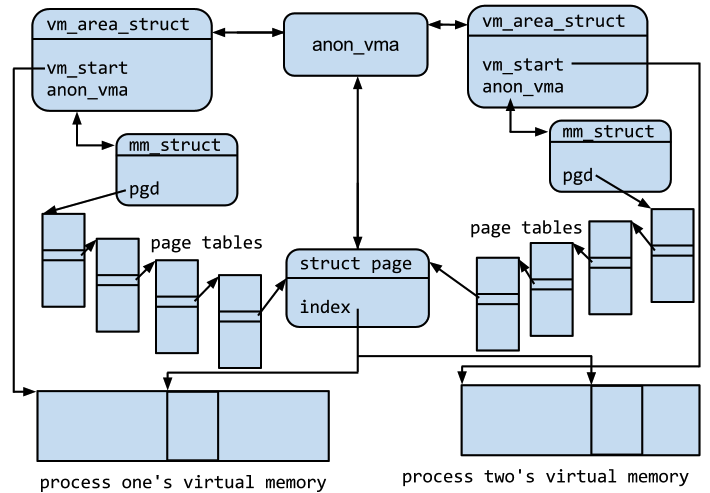
\includegraphics[scale=.33]{anon_vma.png}
\caption{Data structure relationships associated with object-based reverse
mapping. Two processes map virtual memory to the same page read only (possibly
at different addresses). In order for the kernel to swap a given page to disk,
object-based reverse mapping assumes each process maps the page to
\mbox{{\tt vm\_area\_struct->start\_addr} + {\tt page->index}} in virtual
memory.}
\label{fig:anon_vma}
\end{figure}

\paragraph{Memory subsystem} Linux supports a wide range of virtual memory
features including memory mapped files, huge pages, and swapping to disk. All
of these features are layered on top of an abstraction for supporting memory
management units of many different processor architectures (e.g. x86\_64,
Alpha). Whereas Determinator's memory management subsystem deals
only with page table management for a single architecture, Linux's memory
subsystem uses more complicated data structures and nontrivial algorithms.
Figure~\ref{fig:anon_vma} demonstrates the complicated data structures associated
with object based reverse mapping~\cite{overlyanon} used to find all processes
that map a given page of memory. From an implementation perspective, Linux's
memory subsystem's complexity presents a potentially formidable challenge in
implementing Determinator's three memory operations ({\tt Zero}, {\tt Copy}, and
{\tt Snap/Merge}).

\iffalse
	\item Challenges
	\begin{itemize}
		\item Address four sources of non-determinism identified by Aviram.
			Determinator addressed these by not adding these features in its OS
			design. Linux already supports these features, so they must be removed
			or restricted.
		\begin{itemize}
			\item ``Semantically-relevant non-deterministic'' inputs should be made
			into controllable explicit I/O.
			\item Programs cannot share state (memory).
			\item Non-deterministic scheduling abstractions: data racy locks must
				be disallowed.
			\item Globally shared namespaces (process IDs) must not be used.
		\end{itemize}
		\item By design, Determinator enforces all but the root process to be
			deterministic, so we must rethink this design aspect.
		\item We would like to support legacy Linux programs (we don't want to
			have to rewrite init and every other popular Linux program).
		\item Linux process model allows reparenting and children to outlive
			parents, must be disallowed. Processes have more complicated relationships:
			thread ID, process ID, group ID, session ID.
		\item Linux supports signals, System V IPC, disk-backed file system which must
			be disabled for deterministic processes.
		\item Memory subsystem uses more complicated abstractions for managing a
			process's memory: list of contiguous memory regions with complicated
			rules, generic four level page table, non-trivial locking rules, and
			disk-swappable private pages. Also supports huge pages (2MB) and page
			deduping ``kernel samepage merging'' - these all complicate memory
			management considerations.
		\item Specific example: copy-on-write can only be employed when two mm\_structs
			have vm\_area\_regions with matching start and end addresses. Reason: page
			frame reclaiming assumes a page has the same offset from the vm\_area\_region
			start address in every page table entry.
\fi

\begin{figure*}[ht]
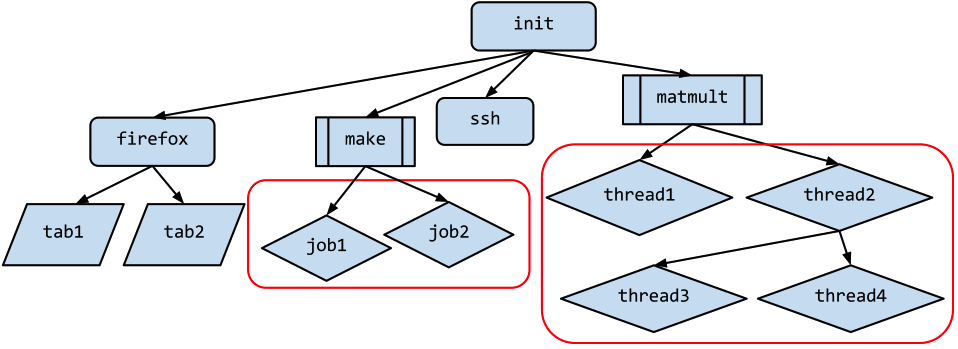
\includegraphics[scale=.5]{proc-diagram.png}
\caption{Illustration of the hybrid process model with two deterministic process
groups. Legacy nondeterministic processes ({\tt firefox},
{\tt ssh}) run as children of {\tt init}. {\tt make} and {\tt matmult} are
masters of deterministic applications. The deterministic children (the diamond
processes) are isolated from the rest of the system.}
\label{fig:proc-diagram}
\end{figure*}

\paragraph{Standard C Library} Many Linux applications written in C use
the standard C library. This library in large part functions as a wrapper around
legacy Linux syscalls and thus is highly nondeterministic. Whereas some
functions, such as {\tt strlen()} might not use nondeterministic syscalls, many
other functions do use nondeterministic syscalls (e.g. {\tt printf()}). Thus,
deterministic programs may be forced to use a completely different library.
Moreover, libraries in Linux are often linked dynamically with shared
libraries, but since Determinator does not provide any native kernel support for
dynamic linking, we may lose the ability to dynamically link shared libraries.

\iffalse
		\item Standard C library implementation obviously relies on legacy syscalls.
			We can either try to run our deterministic user library alongside this
			legacy library, or write our own entirely from scratch.
	\end{itemize}
\fi

\subsection{High level approach}

To address concerns about Linux's more flexible process model, we present a
\emph{hybrid process model}. A Linux process invokes the {\tt dput()} syscall
(introduced below) to become a
\emph{master} process, akin to Determinator's lone root process. This master
process has full access to the legacy Linux kernel API, with some minor
restrictions noted below. Master processes then create \emph{deterministic}
children. We call this master process and its entire subtree a
\emph{deterministic process group}. Within this process group, processes abide
by Determinator's nesting rules (e.g. children cannot outlive parents).
Legacy Linux applications run alongside deterministic applications with
absolutely no kernel restrictions. In some sense, each deterministic application
resembles an entire Determinator ``virtual machine'' of sorts.

We also add three new syscalls, {\tt dput()}, {\tt dget()}, and {\tt dret()}
and restrict deterministic processes to only use the new syscalls. These
syscalls function exactly as their Determinator counterparts, excepting cluster
support, the copy (grand)child subtree option, and instruction count limits.
By restricting deterministic processes to these three syscalls, we can nearly
remove all sources of nondeterminism; we only have to modify the kernel to
ignore all signals sent to deterministic processes, and thus we have effectively
blocked all sources of nondeterminism. Figure \ref{fig:proc-diagram} illustrates
the hybrid process model in a hypothetical environment.

\iffalse
-- where to put root process limits (no KSM, no memadvise for huge pages)
We limit root processes in certain ways
\fi

\iffalse
	\item High level approach
	\begin{itemize}
		\item Hybrid process model: a Linux process becomes a root (akin to the
			lone Determinator root process) process via syscall. This process has
			(nearly) full access to Linux's syscall API. Restrictions explained
			later. Children of root, called deterministic, abide by Determinator's
			strict process hierarchy. Deterministic processes can only communicate
			with their parent and children using the three syscall API. All other
			Linux processes shall be called legacy; these processes can have no
			interaction with deterministic processes (signals, etc) except explicitly
			through the root process.
		\item Deterministic processes can only call three syscalls: dput(), dget(),
			and dret(); this restriction is nearly enough to block all
			non-deterministic inputs. All user generated signals to deterministic
			processes are ignored.
		\item Implement the three syscalls as described by Aviram (at a high level).
\fi

At the expense of predictability, but without harming determinism, master
processes can use nonblocking {\tt dput()} and {\tt dget()} (invoked with a 
special flag) to poll whether or not the child process has reached a
synchronization point yet. We have to chosen to allow this, since some parallel
applications fail to exploit optimal concurrency in Determinator's design.
Since threads are responsible for scheduling children, a CPU might become
available while the scheduler thread remains blocked waiting for another thread
to finish. Applications that use the nonblocking syscalls
can still log schedule sequences to reproduce program output in a deterministic
fashion.

We also allow signals to reach master processes. Master processes can
specify a set of signals that can interrupt a blocking {\tt dput()} or
{\tt dget()}. Allowing signals for master processes again introduces
nondeterminism, but we note that the master can control the signals and write
them to a log file for replay. We also note 
the usefulness of signals: terminal operators can send a {\tt SIGINT} to kill
an application immediately.

Once this kernel work is done, we begin work on a C user library. Deterministic
applications won't use the standard C library, because many library calls
invoke disallowed legacy syscalls. Unfortunately, many functions must be
rewritten (e.g. {\tt sprintf()}, {\tt strlen()}).

To increase the usefulness of the system, we provide an in-memory file system
just as Determinator does. Whereas Determinator's file system uses fixed file
size~\cite{Aviram10cloud}, our file system design is based on the BSD
Fast File System~\cite{mckusick1984fast}. Our file system is organized as a
rooted tree and supports hard linking, dynamic file sizes that can grow up to
1GB, and better resource management (inodes, data blocks). Since a disk-backed
file system is standard on Linux systems, master processes can save and load the
in-memory file system to disk to provide persistence.

\iffalse
		\item Once kernel work is finished, write user library to wrap around the
			three syscalls. Provide familiar fork(), wait(), and exec(), among others.
		\item The user library will be built from scratch: absolutely no libc. This
			gives us freedom in designing the in memory file system and implementations 
			of malloc(), etc. This user library should still behave as closely to the
			familiar C standard API (malloc, read, printf...).
		\item Write in memory file system with similar high level functionality as 
			that in Determinator. This file system also keeps track of standard input
			and output.
	\end{itemize}
\end{itemize}

\fi

\endinput

